 
\chapter{Bayesian Nonparametric Hidden Markov Models}
\label{chap:seven}

The dynamic network models of the Chapter~\ref{chap:six} introduced 
an important idea --- the notion of a time-varying latent state. While 
we did not explicitly frame it in these terms, the dynamic weight 
matrices are an example of a latent population state. There, the state had 
a concrete biophysical interpretation and was imbued with dynamics derived from synaptic plasticity, 
but in general, latent state space models need not be tied 
to specific biophysical phenomena. In this chapter, we explore a very common 
state space model, the hidden Markov model (HMM), which can   
model neural spike trains as a progression of discrete latent states.
By relating these states to externally measured covariates,
we can gain insight into the computations performed by neural circuits.

Hidden Markov models have found numerous applications in neural
modeling.  Recently, \citet{latimer2015single} have used HMMs to
argue that decision-making related activity in macaque lateral
intraparietal (LIP) area is better characterized by a discrete step
between ``undecided'' and ``decided'' states. Similarly, \citet{miller2010stochastic}
have used HMMs to model the dynamics of neural activity during taste 
processing and decision making. In modeling the activity in hippocampal
place cells, \citet{Chen12a, Chen14} have used HMMs to interrogate
discrete states of hippocampal activity and reconstruct topological 
maps of the environment from neural activity. This chapter provides
further analysis of the same hippocampal dataset, which was also used
in Chapters~\ref{chap:three} and~\ref{chap:five}.

A major challenge with using HMMs in practice is determining the
number of latent states. It is common to fit models of varying
dimensionality and compare them on the basis of a cross-validation
metric, such as the predictive log-likelihood assigned to held-out
data. However, this approach has a number of drawbacks. First, it can
be computationally expensive to fit and compare a sequence of
models. Second, it makes inefficient use of the data since we can only
use a fraction of the data to train the model. While this is primarily
a concern in the ``small data'' regime, it is still relevant to neural
data analysis. Third, as with basic mixture models, the standard model
does not explicitly penalize duplicate states. This penalty is only
implicitly enforced through cross-validation. In terms of
interpretability, it is desirable to incorporate an explicit penalty
on excess states.


Here we extend the preceding work and consider a \emph{Bayesian nonparametric} approach.  The Bayesian nonparametric approach brings
additional flexibility to the probabilistic model, which allows us to
model the complex structure of neural data
\citep{Teh10,Wood08,Shalchyan14}.  Specifically, we use a hierarchical
Dirichlet process hidden Markov model (HDP-HMM) \citep{Teh06}, which
extends the finite-state HMM with an HDP prior that theoretically
allows a countably infinite number of states.  The Dirichlet process
provides a nonparametric prior over atomic probability measures with
support for a countably infinite number of outcomes. This is a natural
way to model distributions over infinitely many states, e.g. to model
the rows of a transition matrix.  The \emph{hierarchical} part of the
HDP prior allows sharing between the rows. Even though these priors
support infinitely many states, we can still perform efficient
inference by leveraging truncation methods and constructive
definitions of the HDP that only instantiate variables for states that
are visited in the data.

Nevertheless, inference in Bayesian nonparametric models can be
finicky.  Hyperparameters of the HDP prior can have a strong effect,
as can the particular choice of inference algorithm. Here we provide a
thorough assessment of various inference approaches. We consider both
MCMC and variational inference algorithms. For MCMC, we adapt the
Gibbs sampling approach of \citep{Teh06}, and consider various methods
of inferring hyperparameters.

We test the statistical model and inference methods with both
simulation data and experimental data. The latter consists of a
recording of rat dorsal hippocampal ensemble spike activity during
open field navigation. Using a decoding analysis and predictive
likelihood, we verify and compare the performance of the proposed
Bayesian inference algorithms. 

\section{Probabilistic Model}

First we present a standard Bayesian hidden Markov model with a fixed,
finite number of states. We introduce notation and prior distributions
for the various model parameters. Then we extend this to the nonparametric
case with a countably infinite number of latent states.

\subsection{Parametric Hidden Markov Models} 

Consider a finite $K$-state HMM applied to population spiking activity
from a population of $N$ neurons. We assume that the discrete latent
state follows a first-order Markov chain ${\bz = \left[ z_1, \ldots,
    z_T\right]}$ with~$z_t \in \{1, \ldots, K\}$, and second, the
spike counts of individual neurons at time $t$ follow a Poisson
distribution whose rate depends on the latent state,~$z_t$. This is
summarized in the following probabilistic model:
\begin{align}
  p(\bS, \bz \given \bpi^{(0)}, \bP, \bLambda) 
  &= p(z_1\given \bpi) \prod_{t=2}^T p(z_t \given z_{t-1}, \bP) 
  \prod_{t=1}^T p(\bs_t \given z_t, \bLambda),
\end{align}
where
\begin{align*}
  p(z_1 \given \bpi^{(0)}) &= \distCategorical(z_1 \given \bpi^{(0)}), \\
  p(z_t \given z_{t-1}, \bP) &= \distCategorical(z_t \given \bpi^{(z_{t-1})}), \\
  p(\bs_t \given z_t, \bLambda) &= \prod_{n=1}^N \distPoisson(s_{t,n} \given \lambda_{z_t,n}).
\end{align*}
Here,~$\bpi^{(0)} \in [0,1]^K$ is a discrete probability distribution over
initial states, and
\begin{align*}
  \bP &=
        \begin{bmatrix}
          \text{---} &  \bpi^{(1)}  & \text{---} \\
            &  \vdots &   \\
          \text{---} &  \bpi^{(K)}  & \text{---}
        \end{bmatrix},
\end{align*}
is a~${K \times K}$ transition matrix where the row,~${\bpi^{(k)} \in
  [0,1]^K}$, specify a discrete conditional distribution over~$z_t$
given that~${z_{t-1}=k}$. 
The state-conditional firing rates are collected in the matrix,
\begin{align*}
  \bLambda 
  &=
    \begin{bmatrix}
      \text{---} &  \blambda^{(1)}  & \text{---} \\
      &  \vdots &   \\
      \text{---} &  \blambda^{(K)}  & \text{---}
    \end{bmatrix}
   =
    \begin{bmatrix}
      \lambda_{1,1} & \ldots  & \lambda_{1,N}  \\
      \vdots        &         & \vdots  \\
      \lambda_{K,1} &  \ldots & \lambda_{K,N} 
    \end{bmatrix}, 
\end{align*}

% Finally, $\log p(\bS \given \bz, \bpi^{(0)}, \bP, \bLambda)$ defines the observed data log
% likelihood given the hidden state sequence $\bz$.
% The hidden variables $\bz$ are treated as the
% missing data, ${\bS}$ as the observed (incomplete) data, and
% their combination $\{\bS, \bz\}$ as the complete data.

In a Bayesian version of this model,  we introduce prior distributions over
the parameters. We use the following prior distributions,
\begin{align*}
  \alpha_0 &\sim \distGamma(a_{\alpha_0}, 1.0) \\
  \bpi^{(0)} &\sim \distDirichlet(\alpha_0\bone),\\
  \bpi^{(k)} &\sim \distDirichlet(\alpha_0\bone), \\
  \lambda_{k,n} &\sim \distGamma(\kappa_n,\nu_n).
\end{align*}
where gamma prior on firing rates has neuron-specific shape parameters,
$\kappa_n$, and scale parameters, $\nu_n$.

\subsection{Nonparametric Hidden Markov Models}

Model selection is an important issue for statistical modeling and
data analysis.  Here we extend the finite-state HMM to an
HDP-HMM: a Bayesian nonparametric extension of the HMM that allows for
a potentially infinite number of hidden states \citep{Teh06,
  Beal02}. The HDP-HMM treats the priors via a stochastic
process. Instead of imposing a Dirichlet prior distribution on the
rows of the finite state transition matrix $\bP$, we use a HDP that
allows for a countably infinite number of states.

Specifically, we sample a distribution over latent states,~$G_0$, from
a Dirichlet process (DP) \citep{Ferguson73}
prior,~${G_0\sim \DP(\gamma,H)}$, where~$\gamma$ is the
concentration parameter and~$H$ is the base measure.  Moreover, we
place a prior distribution over the concentration parameter,~$\gamma
\sim \distGamma(a_{\gamma}, 1.0)$.  Given the concentration, one may
sample from the DP via the ``stick-breaking construction''
\citep{Sethuraman94}. First, sample the stick-breaking
weights,~$\bbeta$,
\begin{eqnarray}                                   
\widetilde{\beta}_{k}\sim \distBeta(1,\gamma), \;\;\; \beta_{k}=\widetilde{\beta}_{k}\prod_{j=1}^{k-1}\Big(1-\beta_{j}\Big)
\label{stick1}
\end{eqnarray}
where~$\beta_1 = \widetilde{\beta}_1$,~$\sum_{k=1}^\infty \beta_{k}=1$.

The stick-breaking construction of (\ref{stick1}) is sometimes denoted
as~${\bbeta \sim \mathrm{GEM}(\gamma)}$, after Griffiths, Engen, and
McCloskey \citep{Ewens90}.  The name ``stick-breaking'' comes from the
interpretation of $\beta_k$ as the length of the piece of a
unit-length stick assigned to the $k$-th value.  After the first $k-1$
values having their portions assigned, the length of the remainder of
the stick is broken according to a sample $\widetilde{\beta}_k$ from a
beta distribution, and ${\beta}_k$ indicates the portion of the
remainder to be assigned to the $k$-th value. Therefore, the
stick-breaking process $\mathrm{GEM}(\gamma)$ also defines a DP---
smaller values of $\gamma$ will lead to larger values
of~$\widetilde{\beta}_k$, which means most of the probability mass
will be allocated to the first ``sticks,'' i.e. the small values
of~$k$.

After sampling~$\bbeta$, we next sample the latent state variables, in
this case~${\blambda^{(k)}}$, from the base measure~$H$. For us,~$H$ is 
simply a set of independent gamma distributions for each neuron.
Our draw from
the~${\DP(\gamma,H)}$ prior is then given by
\begin{align*}
G_0(\blambda)=\sum_{k=1}^\infty \beta_k \, \delta_{\blambda^{(k)}}(\blambda).
\end{align*}
Thus, the stick breaking construction makes clear that draws from a
Dirichlet process distribution are discrete with probability one.

Given a countably infinite set of shared states, we may then sample
the rows of the transition
matrix,~${\bpi^{(k)}\sim\DP(\alpha_0,\bbeta)}$. We place the
same prior over~$\bpi^{(0)}$.  The base measure in this case is~$\bbeta$, a
countably infinite vector of stick-breaking weights, that serves as
the mean of the DP prior over the rows of~$\bP$. The concentration
parameter,~$\alpha_0$, governs how concentrated the rows are about the
mean. Since the base measure~$\bbeta$ is discrete, each row of~$\bP$
will be able to ``see'' the same set of states. By contrast, if we
remove the HDP prior and treat each row of~$\bP$ as an independent draw
from a DP with base measure~$H$, each row would see a disjoint set of
states with probability one. In other words, the hierarchical prior is
required to provide a discrete (but countably infinite) set of latent
states for the HMM.

\section{Markov chain Monte Carlo (MCMC) Inference}


Several MCMC-based inference methods have been developed for the
HDP-HMM \citep{Teh06,van08}. Some of these previous works use a
collapsed Gibbs sampler in which the transition matrix~$P$ and the
observation parameters~$\bLambda$ are integrated out
\citep{Teh06,van08}. In this work, however, we use a ``weak limit''
approximation in which the DP prior is approximated with a symmetric
Dirichlet prior. Specifically, we let
\begin{align}
\label{eq:hdphmm_trans}
\gamma &\sim \distGamma(a_\gamma, 1) \\
\nonumber \alpha_0 &\sim \distGamma(a_{\alpha_0}, 1) \\
\nonumber \bbeta \given \gamma &\sim \distDirichlet(\gamma/K_{\mathsf{max}}, \ldots, \gamma/K_{\mathsf{max}}), \\
\nonumber \bpi^{(0)} \given \alpha_0, \bbeta &\sim \distDirichlet(\alpha_0 \beta_1, \ldots, \alpha_0 \beta_{K_{\mathsf{max}}}), \\
\nonumber \bpi^{(k)} \given \alpha_0, \bbeta &\sim \distDirichlet(\alpha_0 \beta_1, \ldots, \alpha_0 \beta_{K_{\mathsf{max}}}).
\end{align}
where $K_{\mathsf{max}}$ denotes a truncation level for approximating the infinity.  It can be
shown that this prior will weakly converge to the DP prior as the
dimensionality of the Dirichlet distribution approaches infinity
\citep{Johnson14, Ishwaran02}. With this approximation we can
capitalize on forward-backward sampling algorithms to jointly update
the latent states~$\bz$.

Previous work has typically been presented with Gaussian or
multinomial likelihood models, with the acknowledgement that the same
methods work with any exponential family likelihood when the base
measure $H$ is a conjugate prior.  Here we present the Gibbs sampling
algorithm of~\citep{Teh06} for the HDP-HMM applied to the special case
of independent Poisson observations, and we derive Hamiltonian Monte
Carlo (HMC) transitions to sample the neuron-specific hyperparameters of
the firing rate priors.

We begin by defining Gibbs updates for the neuronal firing
rates~$\bLambda$. Since we are using gamma priors with independent
Poisson observations, the model is fully conjugate and simple Gibbs
updates suffice. Therefore, we have
\begin{align*}
\lambda_{k,n} \given \bS, \bz 
  &\sim \distGamma \left(
    \kappa_n + \sum_{t=1}^T s_{t,n} \, \bbI[z_t=k], \; 
    \nu_n + \sum_{t=1}^T \bbI[z_t=k]
    \right).
\end{align*}

Under the weak limit approximation the priors on~$\bpi^{(k)}$
and~$\bpi^{(0)}$ reduce to Dirichlet distributions, which are also conjugate
with the finite HMM. Hence we can derive conjugate Gibbs updates for
these parameters as well. They take the form:
\begin{align*}
  \bpi^{(0)} \given \alpha_0, \bbeta &\sim \distDirichlet\left(\alpha_0\bbeta + \bone_{z_1}\right),\\
  \bpi^{(k)} \given \alpha_0, \bbeta &\sim \distDirichlet\left(\alpha_0\bbeta + \bn_{k}\right),\\
  n_{i,j}&=\sum_{t=1}^{T-1} \bbI[z_t=i] \cdot \bbI[z_{t+1}=j],
\end{align*}
where~$\bone_k$ is a unit vector with a one in the~$k$-th entry.

Conditioned upon the firing rates, the initial state distribution, and
the transition matrix, we can jointly update the latent states of the
HDP-HMM using a {\em forward filtering, backward sampling}
algorithm. Details of this algorithm can be found in
\citet[e.g.]{Johnson14b}; the intuition is that in the backward pass of the
algorithm, we have a conditional distribution over~$z_t$
given~$\bz_{t+1:T}$. We can iteratively sample from these distributions
as we go backward in time to generate a full sample
from~${p(\bz \given \bP, \bpi^{(0)}, \bLambda)}$. Jointly sampling
these latent states allows us to avoid issues with mixing when
individually sampling states that are highly correlated with one
another.

Finally, the Dirichlet parameters~$\bbeta$ and the concentration
parameters~$\alpha_0$ and~$\gamma$ can be updated as
in~\citep{Teh06}. A single iteration of the final algorithm consists
of an update for each parameter of the model. The aforementioned
updates are based upon previous work; one novel direction that we
explore in this work is the sampling of the hyperparameters of the
gamma firing rate priors.

\subsection{Setting firing rate hyperparameters} 
\label{sec:fr_hypers}
We consider three approaches to setting the hyperparameters of the
gamma priors for Poisson firing rates, namely,~${\{\kappa_n,
  \nu_n\}}$ for the $n$-th neuron.  

\begin{itemize}

\item In the first approach, we estimate these parameters using an
  empirical Bayesian (EB) procedure, that is, by maximizing the
  marginal likelihood of the spike counts.  For each neuron, this may be
  easily done using standard maximum likelihood estimation for the
  negative binomial model.  In practice, we found that without
  regularization this approach leads to extreme values of the
  hyperparameters.

 

\item Our second approach samples these hyperparameters using
  Hamiltonian Monte Carlo (HMC) \citep{Neal10}. We note that for fixed
  values of the ``shape'' parameter~$\kappa_n$, the conditional
  distribution of the ``scale'' parameter,~$\nu_n$ is conjugate
  with a gamma prior distribution. However, setting the shape
  parameter \textit{a priori} is challenging because it can have a
  strong influence on the firing rate distribution. HMC allows us to
  jointly sample both the shape and the scale parameters
  simultaneously.

To implement HMC we must have access to both the log probability of
the parameters as well as its gradient. Since both parameters are
restricted to be positive, we instead re-parameterize the problem in
terms of their logs. For neuron~$n$, the conditional log probability
equal to,
\begin{align*}
\mathcal{L} 
  &= \log p(\log \kappa_n, \log \nu_n \given \bLambda) \\
  &= \sum_{k=1}^K \log p(\lambda_{k,n} \given \kappa_n, \nu_n) + \text{const.} \\
  &= \sum_{k=1}^K \kappa_n \log \nu_n - \log \Gamma(\kappa_n) + (\kappa_n - 1) \log \lambda_{k,n} - \nu_n \lambda_{k,n}.
\end{align*}
Taking gradients with respect to both parameters yields,
\begin{align*}
  \frac{\partial \mathcal{L}}{\partial \log \kappa_n} 
  &= \sum_{k=1}^K \left[ \log \nu_n -\Psi(\kappa_n) + \log \lambda_{k,n} \right] \times \kappa_n, \\
  \frac{\partial \mathcal{L}}{\partial \log \nu_n} 
  &= \sum_{k=1}^K \left[ \frac{\kappa_n}{\nu_n}  - \lambda_{k,n} \right] \times \nu_n.
\end{align*}
The HMC algorithm uses these gradients to inform a stochastic walk
over the posterior distribution. With knowledge of the gradients, HMC
can sometimes make large updates to parameters, especially in cases
where the parameters are highly correlated under the posterior.


\item In the final approach, we fix the shape
  hyperparameter,~$\kappa_n$, and infer the scale,~$\nu_n$.  We
  place a gamma prior on the scale,~$\nu_n \sim \distGamma(\mu,
  \nu_0)$. Given~$\kappa_n$, the conditional distribution of the scale
  is
\begin{align*}
  \nu_n \given \kappa_n, \{\lambda_{k,n}\}, \bz  
  &\sim \distGamma\bigg(
    \mu + \sum_{k=1}^K \bbI[n_k > 0] \cdot \kappa_n, \,
    \nu_0 + \sum_{k=1}^K \bbI[n_k > 0] \cdot \lambda_{k,n} \bigg) \\
  n_k &= \sum_{t=1}^T \bbI[z_t=k].
\end{align*}
In the following experiments, we set the shape parameter
be~$\kappa_n=1$, and we set the scale prior parameters to~$\mu=1$
and~$\nu=1$.  This is equivalent to an exponential prior on
rates,~$\lambda_{k,n} \sim \distExponential(\nu_n)$, and an
exponential prior on the scale~$\nu_n \sim \distExponential(1)$.
One could perform cross validation over the shape parameter, but the
exponential prior is a rather weak assumption that enables
fully-Bayesian inference.


\end{itemize}


\subsection{Predictive log likelihood}
With the parameter and hyperparameter inference complete, we evaluate
the performance of our algorithm in terms of its predictive log
likelihood on held-out test data. We approximate the predictive log
likelihood with samples from the posterior distribution generated by
our MCMC algorithm. That is,
\begin{align*}
\log p(\bS_{\mathsf{test}} \given \bS_{1:T}) &= \log \sum_{\bz_{\mathsf{test}}} \int_{\bTheta} p\left(\bS_{\mathsf{test}}, \bz_{\mathsf{test}} \given \btheta \right) \; p\left(\btheta \given \bS_{\mathsf{train}} \right) \mathrm{d}\btheta, \\
&\approx \log \frac{1}{L} \sum_{\ell=1}^L \sum_{\bz_{\mathsf{test}}} p\left(\bS_{\mathsf{test}},  \bz_{\mathsf{test}} \given \btheta^{(\ell)} \right),
\end{align*}
where~${\btheta=(\bLambda, \bP, \bpi^{(0)})}$ and~$\{\btheta^{(\ell)} \}_{\ell=1}^L
\sim p(\btheta \given \bS_{\mathsf{train}})$. The summation over latent state
sequences for the test data is performed with the message-passing
algorithm for HMMs.

\section{Variational Bayesian (VB) inference}



We build upon our previous work \citep{Chen12a,Chen14,Johnson14} to
develop a variational inference algorithm for fitting the HDP-HMM to
hippocampal spike trains. Our objective is to approximate the
posterior distribution of the HDP-HMM with a distribution from a more
tractable family. As usual, we choose a factorized approximation that
allows for tractable optimization of the parameters of the variational
model. Specifically, we let,
\begin{align*}
  p(\bz, \bLambda, \bP, \bpi^{(0)}, \bbeta \given \bS_{1:T}) 
  &\approx q(\bz) \, q(\bLambda) \, q(\bP) \, q(\bpi^{(0)}) \, q(\bbeta).
\end{align*}

Since the independent Poisson observations are conjugate with the
gamma firing rate prior distributions, choosing a set of independent
gamma distributions for~$q(\bLambda)$ allows for simple variational
updates.
\begin{align*}
  q(\bLambda) &= \prod_{k=1}^K \prod_{n=1}^N \distGamma\left(\widetilde{\kappa}_{k,n},\, \widetilde{\nu}_{k,n} \right), \\
  \widetilde{\kappa}_{k,n} &\leftarrow \kappa_n + \sum_{t=1}^T s_{t,n} \mathbb{E}_q\big[\bbI[z_t=k]\big], \\
  \widetilde{\nu}_{k,n} &\leftarrow \nu_n + \sum_{t=1}^T \mathbb{E}_q\big[\bbI[z_t=k]\big].
\end{align*}

Following \citep{Johnson14}, we use a ``direct assignment'' truncation
for the HDP \citep{Bryant12, Liang07}. In this scheme, a truncation
level~$K_{\mathsf{max}}$ is chosen {\it a priori} and~$q(\bz)$ is limited to
support only states~${z_t\in\{1,\ldots, K_{\mathsf{max}}\}}$. The advantage of this
approximation is that conjugacy is retained with~$\bLambda$,~$\bP$,
and~$\bpi^{(0)}$, and the variational approximation~$q(\bz)$ reduces
to
\begin{align*}
q(\bz) &= \mathrm{HMM}(\widetilde{\bP}, \widetilde{\bpi}^{(0)}, \widetilde{\bLambda}), \\
\widetilde{\bP} &= \exp\left\{\mathbb{E}_q[\ln \bP]\right\}, \\
\widetilde{\bpi}^{(0)} &= \exp\left\{\mathbb{E}_q[\ln \bpi^{(0)}]\right\}, \\
\widetilde{\bLambda} &= \exp\left\{\mathbb{E}_q[\ln p(\bS \given \bLambda)]\right\}.
\end{align*}
Expectations~${\mathbb{E}_q[z_t=k]}$ can then be computed using
standard message-passing algorithms for HMMs.

With the direct assignment truncation, the variational factors for the
rows~$\bpi^{(k)}$ and the initial distribution~$\bpi^{(0)}$ are
Dirichlet distributions. Unlike in the finite-state HMM, however,
these Dirichlet factors are now over~${K_{\mathsf{max}}+1}$ dimensions since the final
dimension accounts for all states~${k>K_{\mathsf{max}}}$. Under the HDP prior we
had~${\bpi^{(k)} \sim \DP(\alpha_0 \cdot \bbeta)}$, and under the
truncation the DP parameter becomes~$\alpha_0 \cdot
\bbeta_{1:K_{\mathsf{max}}+1}$.
Again, leveraging the conjugacy of the model, we arrive at the
following variational updates:
\begin{align*}
q(\bP) &= \prod_{k=1}^{K_{\mathsf{max}}} \mathrm{Dir}(\widetilde{\bn}_k), \\
\widetilde{n}_{i,j} &\leftarrow \alpha_0 \beta_j + \mathbb{E}_q[\bbI[z_t=i]\cdot\bbI[z_{t+1}=j]].
\end{align*}
We use an analogous update for~$\bpi^{(0)}$.

The principal drawback of the direct assignment truncation is that the
prior for~$\bbeta$ is no longer conjugate. This could be avoided with
the fully conjugate approach of \citep{Hoffman-2013}, however, this
results in extra bookkeeping and the duplication of states. Instead,
following \citep{Johnson14, Bryant12, Liang07}, we use a point
estimate for this parameter by setting~${q(\bbeta)=\delta_{\bbeta^*}}(\bbeta)$
and use gradient ascent with backtracking line search to update this
parameter during inference.

There are a number of hyperparameters to set for the variational
approach as well. The hyperparameters~$\kappa_n$ and~$\nu_n$ of
gamma prior on firing rates can be set with empirical Bayes, as
above. We resort to cross validation to set the Dirichlet
parameter~$\alpha_0$ and the GEM parameter~$\gamma$.
 

\subsection{Predictive Log Likelihood}
Finally, in order to compute predictive log likelihoods on held-out
test data, we draw multiple samples,~$\{\btheta^{(\ell)}\}_{\ell=1}^L$
for~$\btheta=(\bLambda, \bz, \bP, \bpi^{(0)}, \bbeta)$, from the
variational posterior,~$q$, and approximate the predictive log likelihood as
\begin{align*}
  \ln p(\bS_{\mathsf{test}} \given \bS_{1:T}) 
  &\approx \ln \mathbb{E}_q\left[p(\bS_{\mathsf{test}} \given \btheta)\right] \\
  &\approx \ln \frac{1}{L} \sum_{\ell=1}^L p(\bS_{\mathsf{test}} \given \btheta^{(\ell)}).
\end{align*}

The inference algorithms were implemented based upon the PyHSMM
framework of~\citep{Johnson14b}. The code-base was written in Python
with C offloads for the message passing algorithms.  We have
extended the code-base to perform hyperparameter inference using the
methods described above, and expanded it to tailor to neural spike
train analysis. Our code is publicly available
({\url{https://github.com/slinderman/pyhsmm_spiketrains}}).

% Results
\section{Synthetic Data Experiments}

\begin{figure}[t]
  \centering
  \begin{subfigure}[t]{5.in}
    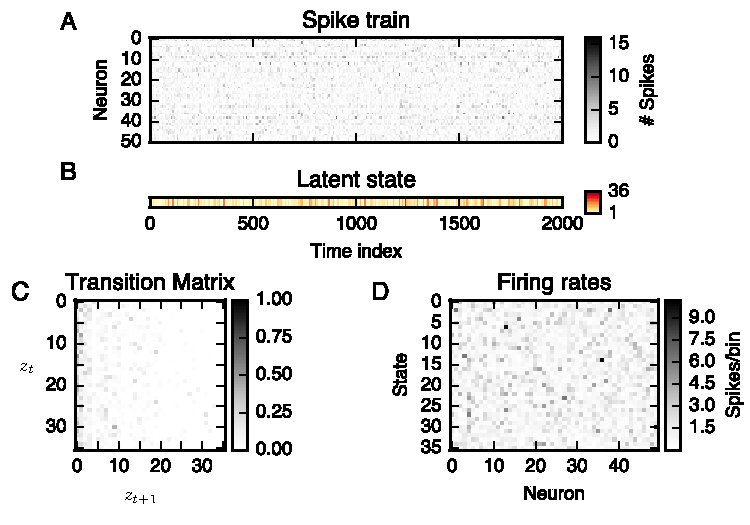
\includegraphics[width=\textwidth]{figures/ch7/Fig1.pdf}
  \end{subfigure}
  \vspace{-.2in}
  \caption[A synthetic dataset drawn from an HDP-HMM]{ An example of a
    synthetic dataset drawn from an HDP-HMM.  (A) Simulated population
    spike trains or spike counts. (B) Inferred latent state
    sequence. (C) Inferred state transition matrix~$\bP$. (D) Inferred
    neuronal firing rate matrix,~$\bLambda$.}
\label{fig1}
\end{figure}

\paragraph{Setup}
\sloppy
 First, we simulate synthetic spike count data using an HDP-HMM with
 ${N=50}$ neurons,~${T=2000}$ time bins, and Dirichlet concentration
 parameters~${\alpha_0=12.0}$ and~${\gamma=12.0}$. These configuration
 yield state sequences that tend to visit $30$--$45$ states. All of
 neuronal firing rate parameters are drawn from a gamma distribution:
 ${\distGamma(\kappa_n=1, \nu_n=1)}$ (with mean $1.0$ and standard
 deviation $1.0$).
 
 An example of one such synthetic dataset is shown in
 Fig.~\ref{fig1}. The states have been ordered according to their
 occupancy (i.e., how many times they are visited during the
 simulation), such that the columns of the transition matrix exhibit a
 decrease in probability as the incoming state number,~$z_{t+1}$,
 increases. This is a characteristic of the HDP-HMM, indicating the
 tendency of the model to reuse states with high occupancy.

We compare six combinations of model, inference algorithm, and
hyperparameter selection approaches: (i) HMM with the correct number
of states, fit by Gibbs sampling with fixed~$\kappa_n=1$; (ii) HMM
with the correct number of states, fit by VB with hyperparameters set
by empirical Bayes; (iii) HDP-HMM fit by Gibbs sampling with
fixed~$\kappa_n=1$; (iv) HDP-HMM fit by Gibbs sampling and HMC for
hyperparameter updates; (v) HDP-HMM fit by MCMC with hyperparameters
set by empirical Bayes; and (vi) HDP-HMM fit by VB with
hyperparameters set by empirical Bayes. For the MCMC methods, we set
gamma priors over the concentration parameters~($\alpha_0$
and~$\gamma$); for the VB methods, we set~$\alpha_0$ and~$\gamma$ to
their true values. Alternatively, they can be selected by cross
validation. We set both the weak limit approximation for MCMC and the
direct assignment truncation level for VB to~${K_{\mathsf{max}}=100}$.

We collect $5000$ samples from the MCMC algorithms and use the last $2000$
for computing predictive log likelihoods. For visualization, we use
the final sample to extract the transition matrix and the firing
rates. The number of samples and the amount of burn-in iterations were
chosen by examining the log probability and parameter traces for
convergence. It is found that the MCMC algorithm converges within
hundreds of iterations. For further convergence diagnosis of a single
Gibbs chain, one may use the autocorrelation tools suggested in
\citep{RafteryLewis92,Cowles96}.

We run the VB algorithm for $200$ steps to guarantee convergence of the
variational lower bound. Again, this is assessed by examining the
variational lower bound and is found to converge to a local maxima
within tens of iterations.


\paragraph{Assessment} 

We use two criteria for result assessment with simulation data.  The
first criterion is based on the Hamming error between the true and
inferred state sequences. To compute this, we first relabel the
inferred states in order to maximize overlap with the true
states. Let~$\bz$ be the true state sequence
and~$\bz'$ be the inferred state sequence. We define the
overlap matrix~$O \in \naturals^{K_{\mathsf{max}} \times K_{\mathsf{max}}}$ whose entries~$O_{i,j}$
is the number of times the true state is~$i$ and the inferred state
is~$j$:
\begin{align*}
O_{i,j} &= \sum_{t=1}^T \bbI[z_t=i] \, \bbI[z'_t=j].
\end{align*}
We use the Hungarian method~\citep{kuhn1955hungarian} to find a
relabeling of the inferred states that maximizes overlap, and then we
measure the Hamming error between the true state
sequence~$\bz$, and the relabeled sequence of inferred
states,~$\widetilde{\bz}'$:
\begin{align}
\label{eq:hamming}
\text{err}(\bz, \widetilde{\bz}') &= \sum_{t=1}^T \bbI[z_t \neq \widetilde{z}'_t].
\end{align}

Table~\ref{tab:synth_hamming} summarizes the Hamming error for all six
models on five synthetic datasets. We see that the HDP-HMM fit via
Gibbs sampling with firing rate hyperparameters set via empirical
Bayes outperforms the other models and inference algorithms on three
of five datasets, but the HDP-HMM with hyperparameter HMC sampling are
very comparable. By contrast, when the models are fit with VB
inference, the inferred state sequences tend to use more than the true
number of states, which results in very poor Hamming error. Similarly,
the HMM fit via Gibbs sampling does not factor in the penalty on
additional states and instead tends to use all states equally,
resulting in high Hamming error.

\begin{table}
  \centering
  \caption[Comparison of Hamming error on synthetic data]{Comparison
    of Hamming error (see Eq.~\ref{eq:hamming}) computed from the same
    nine simulated data sets as above. The VB inference methods tend
    to overestimate the number of states and therefore have much
    higher Hamming error.}
  \begin{tabular}{l|ccccc}
    Dataset & 1 & 2 & 3 & 4 & 5 \\
    \hline
    HMM (Gibbs)     & $9$ & $401$ & $13$ & $24$ & $615$ \\
    HMM (VB)        & $166$ & $290$ & $295$ & $123$ & $124$ \\
    HDP-HMM (Gibbs) & $2$ & $\bf{3}$ & $5$ & $\bf{1}$ & $6$ \\
    HDP-HMM (HMC)   & $3$ & $4$ & $3$ & $2$ & $\bf{4}$ \\
    HDP-HMM (EB)    & $\bf{1}$ & $\bf{3}$ & $\bf{2}$ & $3$ & $12$ \\ 
    HDP-HMM (VB)    & $432$ & $586$ & $340$ & $264$ & $675$ \\
    \hline
  \end{tabular}
  \label{tab:synth_hamming}
\end{table}

The second criterion is the model's predictive log likelihood
(bits/spike) on a held-out sequence of~${T_{\mathsf{test}}=1000}$ time
steps. We compare the predictive log likelihood to that of a set of
independent Poisson processes. Their rates and the corresponding
predictive log likelihood are given by,
\begin{align*}
\widehat{\lambda}_n 
  &=\frac{1}{T_{\mathsf{train}}}\sum_{t=1}^{T_{\mathsf{train}}} s_{t,n}, \\
  \log p(\bS_{\mathsf{test}} \given \bS_{\mathsf{train}}) &= \sum_{n=1}^N \left[ -T_{\mathsf{test}} \widehat{\lambda}_n + \sum_{t=1}^{T_{\mathsf{test}}} s_{t,n} \log \widehat{\lambda}_n  \right].
\end{align*}
The improvement obtained by a model is measured in bits, and is
normalized by the number of spikes in the test dataset in order to
obtain comparable units for each of the test datasets.

Table~\ref{tab:synth_pll} summarizes the predictive log likelihood
comparison.  For all five datasets, the HDP-HMM fit via Gibbs sampling
with fixed~$\kappa_n$ performs best, though in general the increase
over fitting the HDP-HMM when using HMC or EB for hyperparameter
selection is small. By contrast, the improvement compared to fitting
with VB inference or using a parametric HMM is quite significant.

Though computation cost is often a major factor with Bayesian
inference, with the optimized PyHSMM package, the models can be fit to
the synthetic data in under $10$ minutes on an Apple MacBook Air. The
runtime necessarily grows the number of neurons and the truncation
limit on the number of latent states. As the model complexity grows,
we must also run our MCMC algorithm for more iterations, which often
motivates the use of variational inference algorithms instead. Given
our optimized implementation and the performance improvements yielded
by MCMC, we opted for a fully-Bayesian approach using MCMC with HMC
for hyperparameter sampling in our subsequent experiments.

\begin{table}
  \centering
  \caption[Comparison of predictive log likelihood on synthetic
    data]{Comparison of predictive log likelihood (bits/spike)
    computed from 9 simulated data sets, measured in bits per spike
    improvement over a baseline of independent, homogeneous Poisson
    processes (the best result in each data set is marked in bold
    font). }
  \begin{tabular}{l|ccccc}
    Dataset & 1 & 2 & 3 & 4 & 5 \\
    \hline
    HMM (Gibbs)     & $0.315$      & $0.300$ & $0.312$ & $0.310$ & $0.250$ \\
    HMM (VB)        & $0.298$      & $0.290$ & $0.313$ & $0.306$ & $0.252$ \\ 
    HDP-HMM (Gibbs) & $\bf{0.323}$ & $\bf{0.307}$ & $\bf{0.321}$ & $\bf{0.318}$ & $\bf{0.259}$ \\
    HDP-HMM (HMC)   & $\bf{0.323}$ & $0.306$ & $0.320$ & $\bf{0.318}$ & $\bf{0.259}$ \\
    HDP-HMM (EB)    & $0.322$      & $0.306$ & $\bf{0.321}$ & $\bf{0.318}$ & $\bf{0.259}$ \\
    HDP-HMM (VB)    & $0.312$      & $0.291$ & $0.309$ & $0.305$ & $0.244$ \\
    \hline
  \end{tabular}
  \label{tab:synth_pll}
\end{table}

 
\begin{figure}[t!]
  \centering
  \begin{subfigure}[t]{5in}
    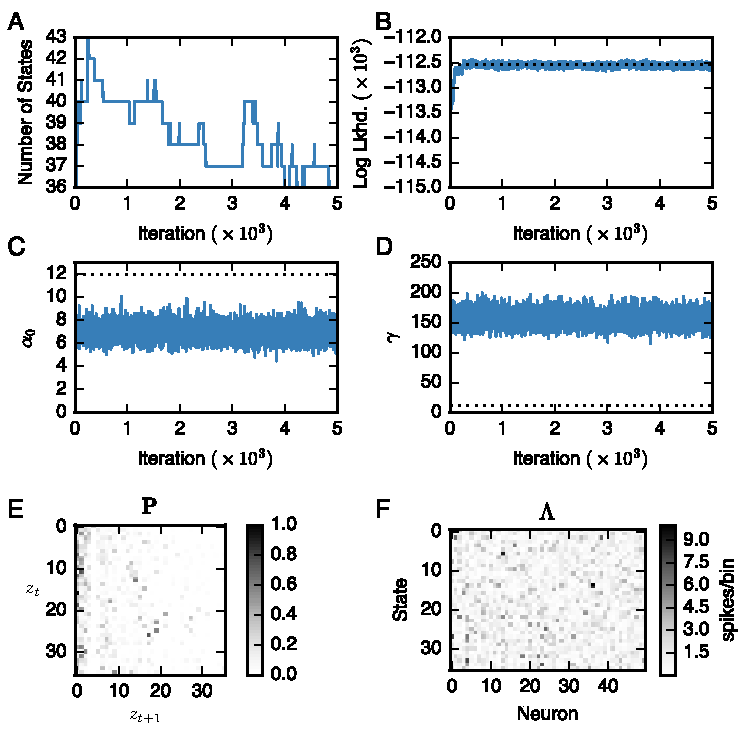
\includegraphics[width=\textwidth]{figures/ch7/Fig2.pdf}
  \end{subfigure}
  \caption[Inference results for an HDP-HMM fit to synthetic
    data]{MCMC state trajectories for an HDP-HMM fit to the synthetic
    dataset shown in Fig.~\ref{fig1}. True values are shown by the
    dotted black lines. The first five iterations of the Markov chain
    are omitted since they differ greatly from the final states. The
    chain quickly converges to nearly the correct number of states (A)
    and achieves close to the true log likelihood (B). (C, D) The
    chain trajectories of hyperparameters $\alpha_0$ and $\gamma$. (E,
    F) Inferred state transition matrix and neuronal firing map drawn
    from the last iteration.  }
  \label{fig2}
\end{figure}

Figure~\ref{fig2} shows example traces from the MCMC combined with HMC
algorithm for the HDP-HMM running on synthetic dataset $1$. This is the
same data from which Fig.~\ref{fig1} is generated. The first $5$ Markov
chain iterations have been omitted to highlight the variation in the
latter samples (the first few iterations rapidly move away from the
initial conditions). We see that the log likelihood of the data
rapidly converges to nearly that of the true model (horizontal dotted
line), and the number of states quickly converges to around~$K=35$.
Note that the nuisance parameters $\alpha_0$ and $\gamma$ do not
converge to the true values --- this is due to the fact that the
solution is insensitive to these parameters or the presence of local
optima.  However, even the concentration parameters are different from
the true values, they are still consistent with the inferred state
transition matrix.

\begin{figure}  
  \centering
  \begin{subfigure}[t]{5in}
    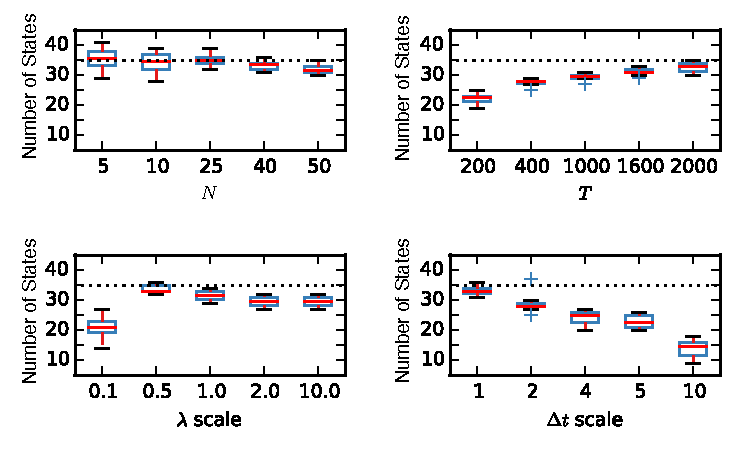
\includegraphics[width=\textwidth]{figures/ch7/Fig3_old.pdf}
  \end{subfigure}
  \caption[Inferred parameters of the HDP-HMM for synthetic data]{In a
    synthetic data experiment, we generated a spike train for a
    population of~$N=50$ neurons
    and~$T_{\textsf{true}}=2000$ time bins. Then we varied the number
    of observed neurons $N$, recording duration $T$, scale of the firing
    rate $\lambda$, temporal bin size $\Delta t$, and measured the
    number of inferred latent states. Horizontal dashed lines indicate
    the ground truth.}
  \label{fig3}
\end{figure}


\paragraph{Sensitivity of the number of latent states} 


To test the sensitivity of the number of inferred states to changes in
the data, we vary a number of parameters and plotted the number of
inferred states in Fig.~\ref{fig3}. In all cases, we use synthetic
dataset~1, shown in Fig.~\ref{fig1}, and HDP-HMMs fit via Gibbs
sampling with fixed~$\kappa_n$. First, we vary the number of
observed neurons,~$N$, and find that the number of inferred states was
relatively stable around the true number of states ($K=35$). By
contrast, as we increase the observed recording length,~$T$, the
number of inferred states increases as well. This is because the true
underlying data actually does visit more states as we simulate it for
longer time. In general, we expect the number of inferred states to
grow with the complexity of the data. Next, we vary the scale of the
firing rate by multiplying the true model's firing rate by a factor
of~$0.1$,~$0.5$, $1.0$, $2.0$, or~$10.0$, and sampling a new spike
count. When the rates are very low, most bins do not contain any
spikes, and hence it is not possible to resolve as many states. By
contrast, when the rate is increased, the number of inferred states is
slightly lower than the true number, which is likely the result of a
slight mismatch with the prior on the firing rate
scale~(parameters~$\mu$ and~$\nu_0$ in
Section~\ref{sec:fr_hypers}). Finally, we considerate the effect of
time bin size by scaling up the bin sizes by factors of~$2$
through~$10$. For example, when scaling by a factor of $2$, we add the
spike counts in each pair of adjacent bins. This has a similar effect
to decreasing the recording length by a factor of $2$, and hence we see
the number of inferred states decrease with bin size.

\section{Hippocampal Place Cells} 

Next, we apply the proposed methods to experimental data of the rat
hippocampus. This is the same dataset studied in previous chapters, but
here we applied additional preprocessing.
The experiments were conducted under the supervision of the
Massachusetts Institute of Technology (MIT) Committee on Animal Care
and followed the NIH guidelines.  The micro-drive arrays containing
multiple tetrodes were implanted above the right dorsal hippocampus of
male Long-Evans rats. The tetrodes were slowly lowered into the brain
reaching the cell layer of CA$1$ two to four weeks following the date of
surgery. Recorded spikes were manually clustered and sorted to obtain
single units using a custom software (XClust, M.A.W.).


For demonstration purpose, an ensemble spike train recording
of~${N=47}$ cells was collected from a single rat for a duration of
$9.8$ minutes.  Once stable hippocampal units were obtained, the rat was
allowed to freely forage in an approximately circular open field
environment (radius: $\sim60$ cm).  We bin the ensemble spike activity
with a bin size of $250$ ms and obtain the population vector $\bz$ in
time.  To identify the period of rodent locomotion during spatial
navigation, we use a velocity threshold ($>10$ cm/s) to select the RUN
epochs and merge them together.  One animal's RUN trajectory and
spatial occupancy are shown in Fig.~\ref{fig4} (left and right panels,
respectively). The empirical probability of a location,~${p(\ell)}$,
is determined by dividing the arena into $220$ bins of equal area ($11$
angular bins and $20$ radial bins) and counting the fraction of time
points in which the rat is in the corresponding bin.

\begin{figure}
\centering
\begin{subfigure}[t]{\textwidth}
\centering
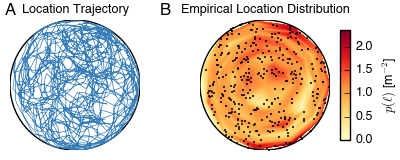
\includegraphics[width=4in]{figures/ch7/Fig4}
\end{subfigure}
\caption[Trajectory of the freely foraging rat during hippocampal
  recording]{One rat's behavioral trajectory (left) and spatial
  occupancy (right) in the open field environment. }
\label{fig4}
\end{figure}

In experimental data analysis, we focus on Bayesian nonparametric
inference for HDP-HMM.  For all methods, we increase the truncation
level to a large value of $K_{\mathsf{max}}=100$.  To discover the model order of the
variational solutions, we use the number of states visited by the most
likely state sequence under the variational posterior. The MCMC
algorithms yield samples of state sequences from which the model order
can be directly counted.


\begin{table}[b]
  \centering
  \caption[Comparison of models on real hippocampal data]{A comparison
    of HMMs, HDP-HMMs, and inference algorithms on the rat hippocampal
    data. Performance is measured in predictive log likelihood and
    mean decoding error on two minutes of held-out test data (the best
    result is marked in bold font).}
  \begin{tabular}{l|cc}
    & Pred. log likelihood (bits/spike) & Decoding error (cm) \\
    \hline 
    HMM ($K=25$)         & $0.712$ & $10.85 \pm 6.43$ \\
    HMM ($K=45$)         & $0.706$ & $10.71 \pm 6.67$\\
    HMM ($K=65$)         & $0.717$ & $11.01 \pm 6.93$\\
    HDP-HMM (Gibbs)      & $\mathbf{0.722}$ & $\mathbf{9.56 \pm 5.31}$ \\
    HDP-HMM (HMC)        & $0.646$ & $9.96 \pm 6.05$\\
    HDP-HMM (EB)         & $0.579$ & $10.81 \pm 6.78$\\
    HDP-HMM (VB)         & $0.602$ & $10.93 \pm 6.24$
  \end{tabular}
  \label{tab:hipp_err}
\end{table}

We perform a quantitative comparison between HMMs, HDP-HMMs, inference
algorithms, and hyperparameter setting algorithms, where performance
is measured in terms of both decoding error and predictive log
likelihood. For both metrics, we train the models on the first
$7.8$~minutes of data and test on the final two minutes of data for
prediction. The results are summarized in Table~\ref{tab:hipp_err}. We
find that the HDP-HMM fit by Gibbs sampling with fixed firing rate
scale~($\kappa_n=1$) again outperforms the competing models in both
measures.

\begin{figure}[t!]
  \centering
  \begin{subfigure}[t]{5in}
    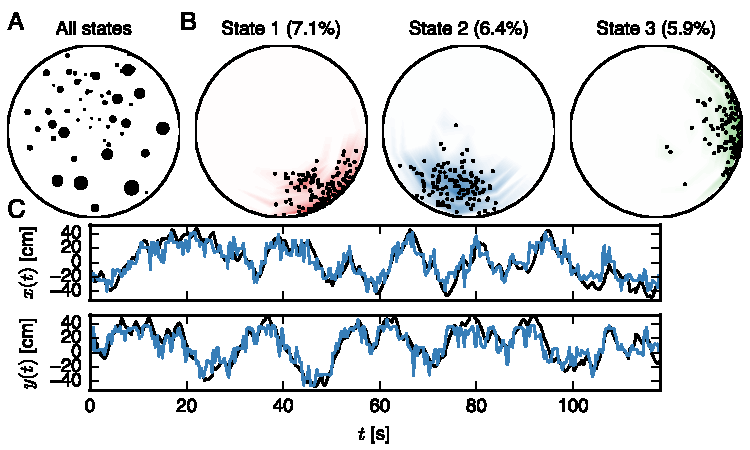
\includegraphics[width=\textwidth]{figures/ch7/Fig5.pdf}
  \end{subfigure}
  \caption[Place fields inferred by an HDP-HMM applied to rat
    hippocampal data]{Estimation result from HDP-HMM (Gibbs) for the
    rat hippocampal ensemble spike data. (A) Estimated state space
    map, where the mean value of the spatial position for each latent
    state is shown by a black dot. The size of the dot is proportional
    to the occupancy of the state.  (B) Probability distributions over
    location corresponding to the top three latent states, measured by
    state occupancy. The small black dots indicate the location of the
    animal while in that state, and are used to compute the empirical
    distribution over location indicated by colored shading. (C) The
    true and reconstructed trajectories in Cartesian coordinate. The
    true trajectory is shown in black and the reconstructed trajectory
    is shown in blue. For each time bin, we use the mean location of
    the latent states to determine an estimate of the animal's
    location. }
  \label{fig5}
\end{figure}


\begin{figure}[t!]
  \centering
  \begin{subfigure}[t]{5.0in}
    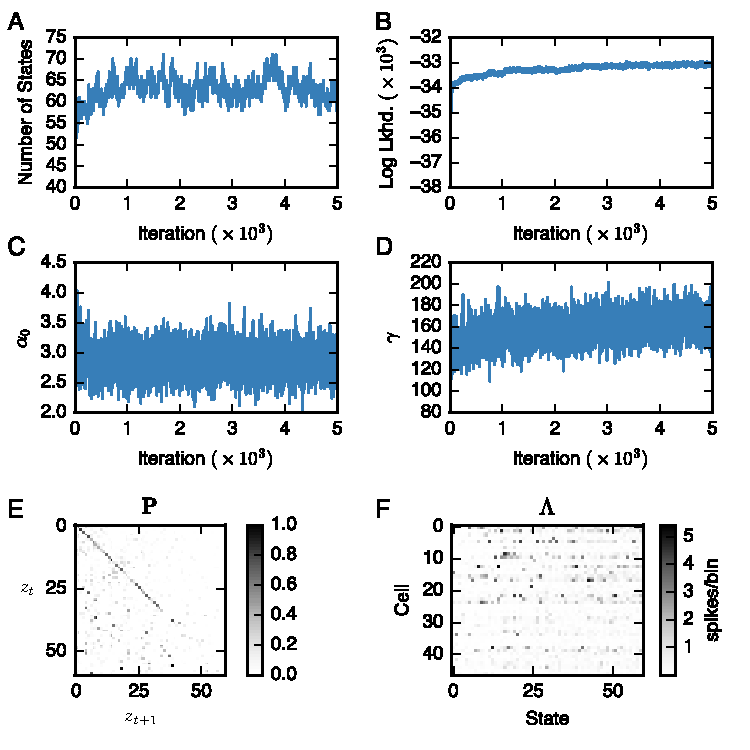
\includegraphics[width=\textwidth]{figures/ch7/Fig6.pdf}
  \end{subfigure}
  \caption[Inferred parameters of the HDP-HMM for hippocampal
    data]{Estimation result from HDP-HMM (Gibbs) for the rat
    hippocampal ensemble spike data. (A) The total number of states
    (solid blue) slowly increases as states are allocated for a small
    number of time bins. The number of states converges after 2500
    iterations. (B) The log likelihood of the training data grows
    consistently as highly specific states are added. (C, D) The
    concentration parameters,~$\alpha_0$ and~$\gamma$ also converge
    after 2500 iterations. (E, F) The inferred state transition matrix
    and firing rate samples drawn from the last iteration.  }
  \label{fig6}
\end{figure}

For the purpose of result assessment, we plot the state-space or
state-location map (Fig.~\ref{fig5}A), which shows the mean value of
the spatial position that each state represented. The size of the
black dot is proportional to the occupancy of the state.  To compute
an ``empirical'' distribution over locations for a given state, we
first compute the posterior distribution over latent states with our
inference algorithms. This gives us a set of
probabilities~$\Pr(z_t=k)$ for all time bins~$t$ and states~$k$. Then
we compute the average location for each state~$k$ by weighting the
animal's location,~$(x_t,y_t)$ by the probability that the animal was
in state~$k$ at time~$t$. Summing over time yields a weighted set of
locations, which we then bin into equal-area arcs and normalize to get
an empirical distribution over locations for each state~$k$.

The empirical location distribution for the top three states as
measured by occupancy are shown in Fig.~\ref{fig5}B). In
Fig.~\ref{fig5}C, we show the estimated animal's spatial trajectories
in black, along with the reconstructed location in from the HDP-HMM
with Gibbs sampling in blue. To reconstruct the position, we use the
mean of each latent state's location distribution weighted by the
marginal probability of that state under the HDP-HMM. That is,
\begin{align*}
\hat{x}_t = \sum_{k=1}^K \bar{x}_k \Pr(\bz_t=k), \qquad
\hat{y}_t = \sum_{k=1}^K  \bar{y}_k \Pr(\bz_t=k),
\end{align*}
where~$\bar{x}_k$ and~$\bar{y}_k$ denote the average location of the
rat while in inferred state~$k$ (corresponding to the black dots in
Fig.~\ref{fig5}A). Note that the animal's position is not used in
model inference, only during result assessment. In the illustrated
example (HDP-HMM with MCMC+HMC), the mean reconstruction error in
Euclidean distance is $9.07$ cm.



As the parameter sample traces in Fig.~\ref{fig6} show, the Markov
chain converges in around $2500$ iterations. After this point, the total
number of states stabilizes to around~$65$.  The concentration
parameters~$\alpha_0$ and~$\gamma$ converge within a similar number of
iterations.  Finally, we show the transition matrix~$\bP$ and firing
rate matrix~$\bLambda$ obtained from the final Markov chain sample.


% Effect of hyperparameters
\begin{figure}[t!]
  \centering
  \begin{subfigure}[t]{5in}
    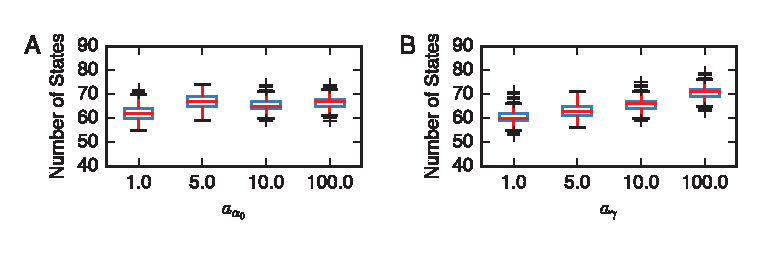
\includegraphics[width=\textwidth]{figures/ch7/Fig7}
  \end{subfigure}
  \caption[Effect of concentration hyperparameters]{Measuring the
    effect of concentration hyperparameters on the number of inferred
    latent states. We find that the concentration hyperparameters of
    the gamma priors on the concentration parameters,~$\alpha_0$
    and~$\gamma$, have a minimal effect.}
  \label{fig7}
\end{figure}



We again evaluated the sensitivity of these model fits to the choice
of hyperparameters. For the HDP-HMM fit via Gibbs sampling with
fixed~$\kappa_n$, the primary hyperparameters of interest are the
concentration hyperparameters,~$a_{\alpha_0}$ and~$a_{\gamma}$ in
Eq.~\ref{eq:hdphmm_trans}, where we have assumed $ \alpha_0 \sim
\distGamma(a_{\alpha_0}, 1)$ and $ \gamma \sim \distGamma(a_\gamma, 1)
$.  Figure~\ref{fig7} shows the inferred number of states as we vary
these two hyperparameters over orders of magnitude. We found that the
number of inferred states is stable around~$65$, indicating the
performance robustness to the choice of these hyperparameters.

% True and inferred place fields
\begin{figure}[t!]
  \centering
  \begin{subfigure}[t]{5in}
    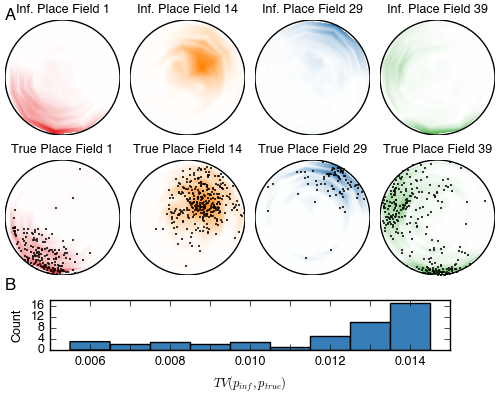
\includegraphics[width=\textwidth]{figures/ch7/Fig8}
  \end{subfigure}
  \caption[True and inferred place field comparison]{Comparison of
    inferred and true place fields for four randomly selected
    hippocampal neurons. The inferred place field (top row) for
    neuron~$n$ is a combination of location distributions for each
    state~$k$ weighted by the inferred firing rates~$\lambda_{k,n}$,
    whereas the true place field (bottom row) for neuron~$n$ is a
    histogram of locations in which neuron~$n$ fires. The black dots
    show the rat's locations used for each histogram. The inferred
    place fields closely match the true place fields. With adequate
    spike data recording, we expect a higher latent state
    dimensionality to yield higher spatial resolution in the inferred
    place fields.}
  \label{fig8}
\end{figure}

Looking into the inferred states, we can reconstruct the ``place
fields'' or ``state fields'' of hippocampal neurons. To do so, we
combine the state-location maps (Fig.~\ref{fig5}B) with the firing
rate of the individual neuron in those states (Fig.~\ref{fig6}F) and
weight by the marginal probability of the latent state. Together,
these give rise to the inferred neuron's place field. Note that,
again, the position data was only used in reconstruction but not in
the inference procedure. Four pairs of inferred and true place fields
are shown in Fig.~\ref{fig8}. On the top row is the inferred place
field; on the bottom is the true place field computed using the
locations of the rat when neuron~$n$ fired shown by black dots.


\section{Extensions}

\paragraph{Hidden Semi-Markovian Models}
A striking feature of the inferred state transition matrix in
Fig.~\ref{fig6}E is that the first $40$ states exhibit strong
self-transitions. This is a common feature of time series and has been
addressed by a number of augmented Markovian models. In particular,
hidden semi-Markovian models (HSMMs) explicitly model the duration of
time spent in each state separately from the rest of the state
transition matrix \citep{Johnson13}. Building this into the model
allows the Dirichlet or HDP prior over state transition vectors to
explain the rest of the transitions, which are often more
similar. Alternatively, ``sticky'' HMMs and HDP-HMMs accomplish a
similar effect \citep{Fox08}.


\paragraph{Dependent Observation Models}
The HMMs in this chapter used conditionally independent Poisson 
observations. Given the latent state, each neuron fires independently 
of the others, and also independently of its previous spike counts.
One way to extend these models is by introducing dependencies in 
the observation models. For example, we can combine the autoregressive
models of previous chapters with the discrete latent states of an 
HMM with a model of the form,
\begin{align*}
  p(\bs_t \given z_t) &= \prod_{n=1}^N \distPoisson(s_{t,n} \given \lambda_{t,n}), \\
  \lambda_{t,n} &= g \left(\psi_n^{(z_t)} + \bw_n^{(z_t)} \bs_{t-1} \right).
\end{align*}
As in previous chapters, this can easily be extended to higher-order 
autoregressive models. 
Expectation-maximization algorithms for this type of model were developed 
by \citet{escola2011hidden}.
Alternatively, we can use the \polyagamma
augmentation schemes of Chapter~\ref{chap:five}, and we have presented
a preliminary versions of this approach in \citet{johnson2015cosyne}.



\paragraph{Input-Output HMMs}
Hidden Markov models are ``open loop'' systems: the next state 
depends only on the previous state.  In practice, it is natural to 
expect that transitions are not only state-dependent but also a 
function of some external variables. For example, in the hippocampus 
where states correspond to actual locations, whether or not the 
rat transitions into a state may depend on instantaneous properties 
of that location. If more complex experimental setups there may 
be food or obstacles in the environment that affect where the rat 
goes next. 

These types of external variables can be modeled with an input-output 
HMM (IOHMM) \citep{bengio1995input}. Suppose we have an external input,
~$\bu_t \in \reals^D$. We can model the transition probability as,
\begin{align*}
\bpi^{(k)} &\propto \exp\{\bpsi^{(k)} + \bW \bu_t\}, \\
\end{align*}
that is, as a ``soft-max'' function of a baseline probability plus a 
weighted combination of input covariates.  Performing inference in this 
type of model is not much more challenging than in the standard HMM.
When sampling the latent states, we simply compute the instantaneous
transition probabilities for each time step. In order to update the 
transition weights,~$\bW$, and the baseline probabilities,~$\bpsi^{(k)}$,
we can either use HMC or our recently developed \polyagamma augmentation scheme for multinomial
models \citep{linderman2015dependent}.


\section{Conclusion}
This chapter explored the idea of dynamic latent states underlying
neural activity. Specifically, we developed Bayesian nonparametric
hidden Markov models (HDP-HMMs) and corresponding MCMC and variational
inference algorithms. Since these models are notoriously sensitive to
hyperparameter settings, we performed a thorough assessment of
inference results on both synthetic data and real recordings from rat
hippocampal place cells.  In the next chapter, we will build on these
ideas, developing more sophisticated latent state space models with a
mix of discrete and continuous latent states. As we will see, HMMs are
only one in a hierarchy of state space models.

